\chapter{Method}


Several hypotheses were tested in this work.
Section \ref{data_pp} gives an overview of how input data was pre-processed.
Section \ref{architecture} describes the technical set up required for running all these experiments and deploying the model to production before delving into the specific experiments and their evaluation in section \ref{exp}.

\hfill \break \noindent
The experiments were conducted in four distinct stages:

 \begin{itemize}
   \item
    Training a baseline model on the rule-based labels to get a sense of the difficulty of this problem.
    Exploring the predictions subjectively.
   \item Building a visual similarity feature and evaluating its results subjectively.
   % Since there is no fundamental difference in the way this model was  trained and evaluated compared to the other classifiers, this is described in section \ref{exp_models} with the others. After this step, employees of the client company labeled products that would become the ground truth dataset. The visual comparison feature was also subjectively evaluated at this stage.
   \item
    Training the independent classifiers to determine best performers (\ref{exp_models}).
    Due to the good perforance of individual models, ensembling was not attempted due to the engineering overhead it would incur.
    Experimenting with different multi-objective training approaches.
   \item Training [TODO] iterations of active learning on the strong predictor (\ref{exp_al}).
 \end{itemize}


 \section{Data Preprocessing}
 \label{data_pp}

There were around a dozen product features that affiliate networks provided.
Most of these features were either categorical or textual,  with just a single numerical feature.
Initially, the data was analysed using Dataprep, a Google Cloud Platform (GCP)  product for data wrangling, which at the time of use was in beta stage.
Dataprep  was used to process a sample of ~800 000 products;  it produced histograms of the values present in each feature column (see appendix \ref{dataprep}).

The histograms revealed that a lot of the input features were mostly empty, but also that many of the inputs that would naturally be considered categorical  had much more unique value in them then one might expect.
For example, each affiliate gives us the textual representation what they consider to be the category of the product,  but  rather than containing a small number of unique tokens, these contained all the full category paths along with the category delimiters, which  varied retailer by retailer (e.g.  it was common to see both ``Shoes > Sneakers'' and ``Shoes // Sneakers'').
Representing these as categorical variables would have blown up the input space, which would have  resulted in more parameters, each parameter having fewer examples to learn from.
Therefore, many such ``categorical''  were actually represented as text, which were tokenised and cleaned appropriately, allowing for better generalisation and smaller models.

There was a single numerical field: price.
This could have been min-max normalised to the range 0 ... 1, however there  was a small number of very high values that would have squash nearly all the other  prices.
Rather than  carefully considering  how to mitigate this,  the input dimension was dropped, because it is not likely to have much predictive value for product classification.
It would be trivial to bring this feature back for a training objective for which it would be much more useful.

A trickier question was how many distinct tokens or categorical values to keep per input column.
Keeping all of them would not have been sensible: there were still large numbers of tokens that appeared only once, often because there were some unwanted formatting characters, misspellings, or incorrect punctuation that caused a token to be considered a separate entity.
There was a single configuration file that dictated which models used which features as input, whether those inputs were represented as textual, categorical, or dense values;  it also determined  the maximum number of unique values/tokens,  and the dimensionality of the embedding.
This configuration file was read by Dataflow during pre-processing  and by TensorFlow during  inference and training, which made experimentation with  different types of models and input representations considerably easier.

Below is a list of input features with information about how they were represented; it also lists the dimensionality of embeddings  for the models which  encoded categorical variables as embedding.

\begin{itemize}[noitemsep]
  \item title - text - max 8000 unique tokens
  \item brand - categorical - max 5000 unique values - 10 embedding dimensions
  \item category - categorical - max 950 unique values - 6 embedding dimensions
  \item rawCategory - text - max 1000 unique tokens
  \item description - text - max 8000 unique tokens
  \item gender - categorical - take all unique tokens
  \item size - categorical - max 100 unique tokens
  \item image - dense vector of 2048 or 1280 dimensions extracted with a 2D CNN
\end{itemize}

\subsection{Category Structure}
\label{cat_tree}

At the time of writing, there were roughly 1300 categories defined in the client database.
Categories were structured in a way that is typical of  e-commerce:  categories can have  child categories, which in turn can have child categories, etc.
In our case, the typical depth of the tree structure was five, i.e. a leaf category often had four parents;  naturally, the tree structure was not balanced, so many branches ended at depth three or four.

Categories can be considered as independent (multi-label) or mutually exclusive (multi-class).
The common way to handle this is to assume categories are mutually exclusive.
With exclusive categories, assigning a label to a product determines its label across all categories, whereas with independent categories a positive label only determines the label across the category in question (and its ancestors in the category tree) - that is roughly a thousand-fold difference in labelling efficiency.
The prediction task is also easier for exclusive classes - rather than needing to predict a probability score above a threshold separately for each class, the model would need to just assign the highest probability to the correct class compared to other classes.
On the other hand, some categories at the client company are inherently ambiguous or even overlapping; the rule-based labels are also independent: a product may be labelled to belong to zero or many categories.
Independent categories are also somewhat easier to handle: with exclusive categories the rule-based and hand-assigned labels would have to be considered as separate training objectives, because the activations from softmax and sigmoid layers that lead to a positive prediction will be different and we can not share the output layer across these two types of labels.


\subsection{Class and Label Imbalance}
\label{label_imbalance}

% HERE

The labels provided by the rule-based system are only positive:  some products are labelled to belong to a given category, but many products that ought to belong to a category are not labelled  accordingly -  but their label still appears to be negative.
This (which we call the label imbalance problem) only exacerbates the class imbalance problem (that most products do not belong to most categories).
As a result the model trained on rule-based labels will certainly underestimate the likelihood of any product belonging to any category.

Still, most positive labels provided by the rule-based system are correct, which means the model should assign higher likelihoods to products that should actually belong to the given class.
Our active learning strategy outlined in section \ref{exp_al} ensures that products around the decision boundary would receive a label - which during the initial rounds of active labelling would be overwhelmingly positive examples.
The first rounds of active labelling should therefore counterbalance the underestimating nature of the pre-trained model; as the model starts to make more ``optimistic'' predictions, the products near the decision boundary should become a more balanced mix of positive and negative examples.

Class imbalance may or may not be an issue after label imbalance has been accounted for.
The worst case scenario is that our model continues to underestimate the likelihood of products belonging to classes, particularly if these are rare classes.
False negatives are not much of our problem in our setting.
There are millions of products that affiliate networks provide, and in any case we can show the average user a tiny fraction of those products, so it is okay if some are left out from some categories and their chance to be seen decreases.
Conversely, false positives will appear unprofessional and reduce user satisfaction.

% If label imbalance remains an issue, one might try to weight the loss function (eq \ref{original_loss}).
% The binary cross entropy loss function we use has two parts per class: the loss incurred for a false positive (FP) and false negative (FN) prediction.
% A weighted version (eq \ref{weighted_loss}) the loss function would wait the false-positive part of the loss function with the fraction of products that belong to that class, and the false negative part of the loss function with the fraction of products that do not belong to that class.
% We do not know how many products actually belong to a given class, and we would need to get this estimate through random sampling.
%
% \begin{align}
%   \label{original_loss} NLL(\theta) &= \sum\limits_{i=1}^N\left[FP + FN )\right] \\
%   \label{weighted_loss} NLLW(\theta) &= \sum\limits_{i=1}^N\left[P(y=1) FP + P(y=0) FN )\right] \\
%   FP &= y_i\log P(y=1|x, \theta) \\
%   FN &= (1-y_i)\log(P(y=0|x, \theta)
% \end{align}
%
% This weighting scheme is motivated by how imbalanced classes in multi-class classification can be handled.
% One option would be to oversample data points from the underrepresented class, but this would incur overhead in computation, and an equivalent method is to  weight the training example based on the class probability, so data points from underrepresented classes get a higher weight.
% As we have several independent output classes, the weighting would have to be done at the loss function level rather than per example.
% Note that the author could not find examples of the weighting scheme in literature, and is therefore not sure whether it is appropriate.

\section{System Architecture}
\label{architecture}

 The following technologies were used to build the system which had to interact with existing services  at the client company:

\begin{itemize}
  \item Apache Airflow (AF) - a Python framework for defining workflows of long-running tasks and dependencies between these tasks.
  \item TensorFlow (TF) - ML framework for Python, capable of defining many kinds of models as a computation graph, and executing this graph locally or in a distributed manner.
  \item ML Engine (MLE) - a GCP service for running TensorFlow models (training, hyperparameter tuning, inference).
  \item Apache Beam - a data processing engine akin akin to Apache Spark and Apache Flink.
  \item Dataflow - a GCP service for executing Apache Beam workloads.
  \item Tensorflow Transform - a Python library with a small set of operations for data preprocessing that can run inside a TensorFlow graph as well as an Apache Beam pipeline.
  \item Google Cloud Storage (GCS) - Google Cloud Platform (GCP) object storage similar to Amazon S3.
  \item ElasticSearch (ES) - a NoSQL database with powerful full-text search and querying capabilities.
  \item RabbitMQ - a message queue, used for transferring data among our microservices (using the Logstash adapter, that can read from and write to (among other things) ElasticSearch and RabbitMQ).
  \item Flask - a simple backend web framework for Python.
  \item Node.js - a JacaScript backend web framework.
  \item React.js - a JavaScript front-end framework for JavaScript.
  \item Redux - a framework for persisting user interface (UI) state and application data in single page applications.
  \item GraphQL - a query language for building flexible APIs
\end{itemize}

Figure \ref{arch_diagram} shows the how data is passed between the main services, and how services and technologies interact.

All product data is stored in ElasticSearch (ES): the rule-based labels, the predictions of the ML system, and evaluation metrics from various train runs.
ES is accessed from the public web application via GraphQL and the ML administration web UI (further referred to just as web UI\footnote{The web UI was initially built with Flask and React by the author as a quick way to get insight about the model, and then re-written as a more feature-rich version by an employee of the client company with Node.js, GraphQL, React and Redux.}).
Data is pulled into the ML pipelines by dumping the results of an ES query to a local file, which is uploaded to GCS.
Updates to the ES index are not done directly, since indexing the updated products is computationally expensive; instead, updates are put on a RabbitMQ queue, which is consumed by Logstash, which in turn updates products in ES at a rate that will not overburden the servers.

All ML training and prediction happens in a batch-oriented way, encapsulated as Airflow pipelines.
Each pipeline is a directed acyclic graph of tasks, where a task can be a shell command or Python function; a pipeline defines dependencies of task execution, which allows us co-ordinate a series of operations that could be executed locally (inside the Docker container running AF) or remotely (such as in a GCP service).
A typical pipeline dumps data locally, uploads it to GCS, schedules a Dataflow job to preprocess data, polls the Dataflow service until the Dataflow job is finished, schedules an ML engine job, polls the MLE service until it has completed, and runs an update process that reads the predictions and evaluation statistics from GCS and sends the updates to the RabbitMQ queue.
Reading updates and sending these to RabbitMQ is done in a parallelised manner (using multiprocessing), since the update process is bottlenecked due to network latency as well as computing the appropriate category path for each product (explained in \ref{cat_tree}).

\begin{figure}
  \hspace*{-0.2\textwidth}
  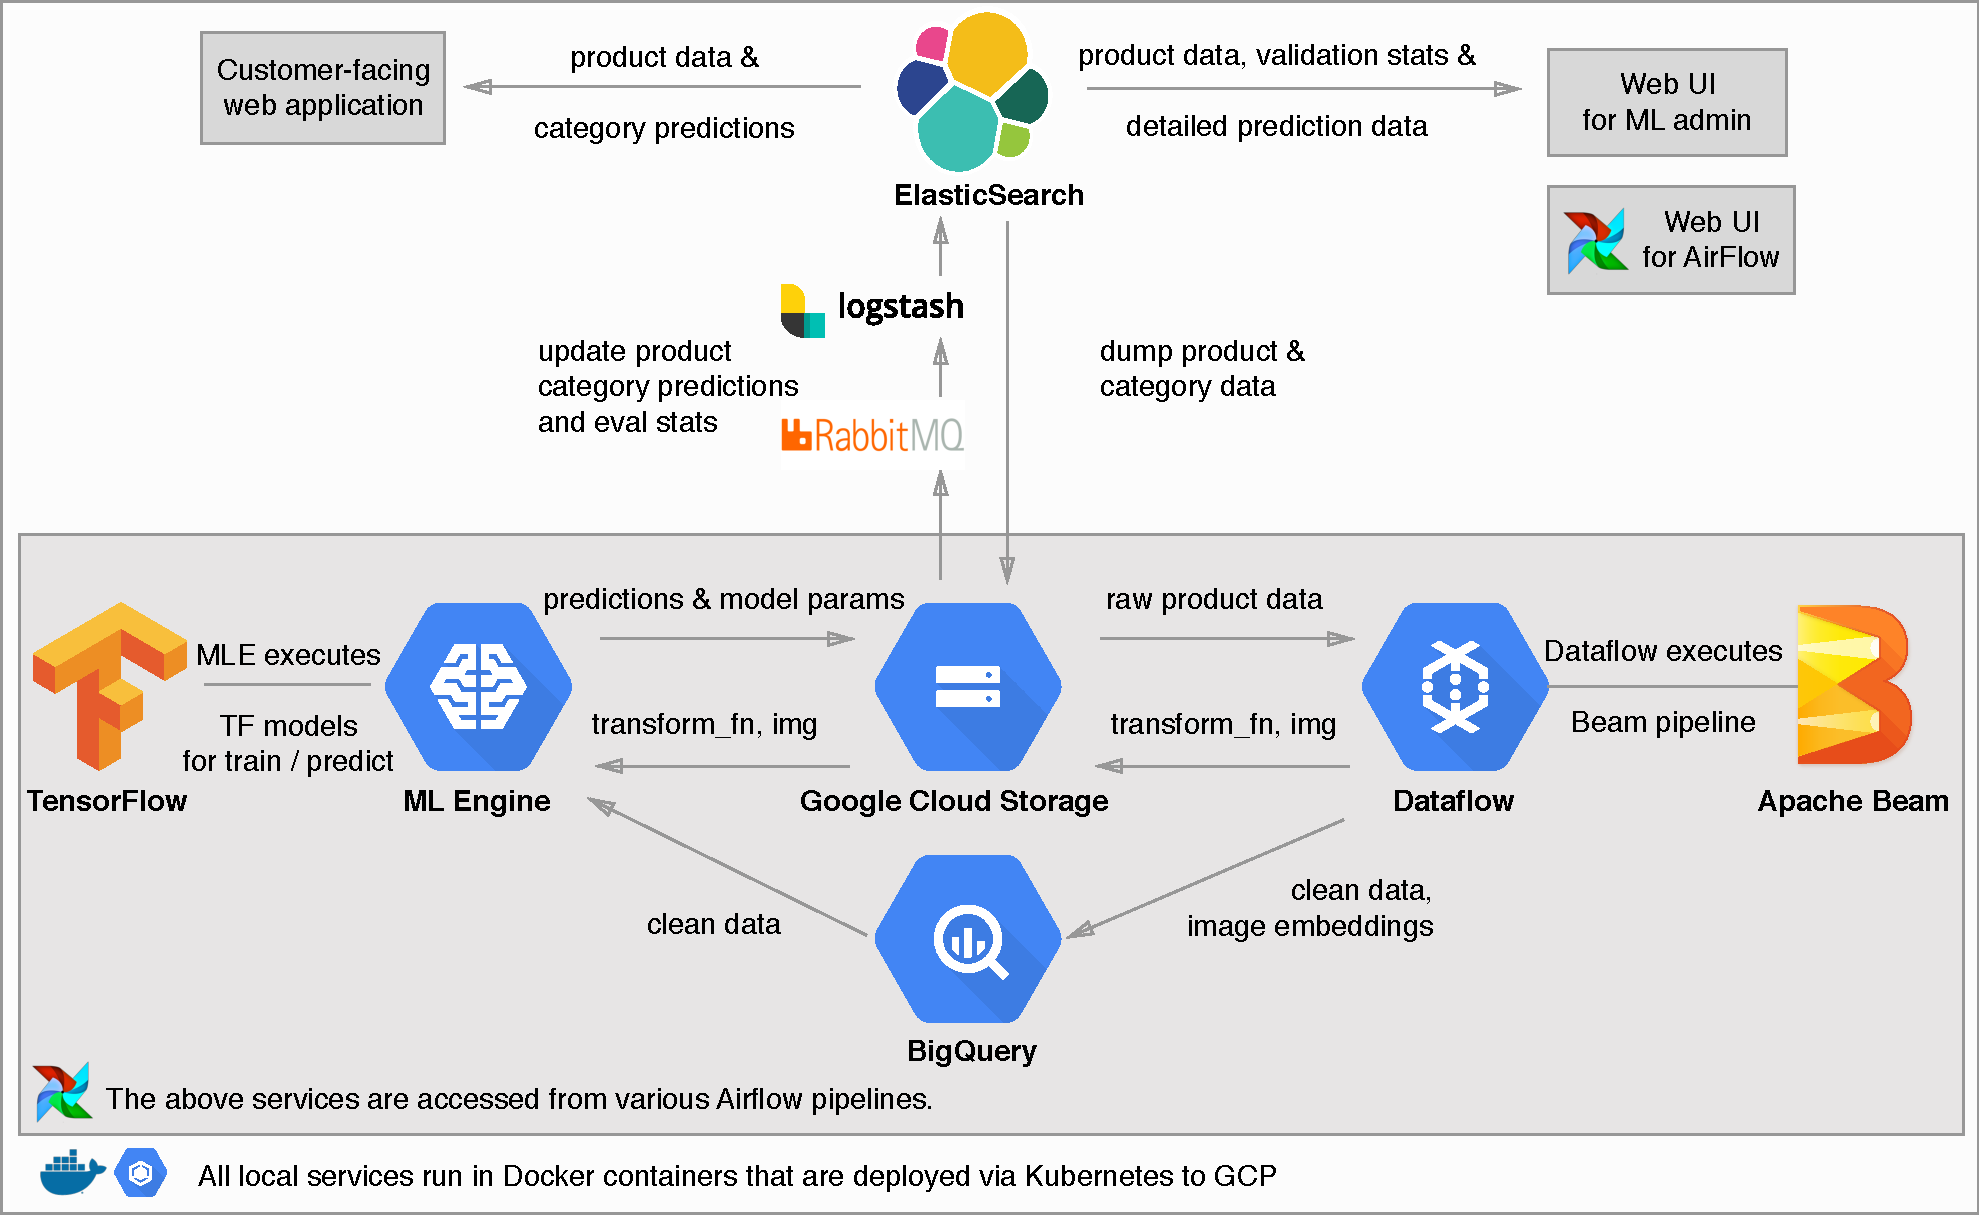
\includegraphics[width=1.4\textwidth]{diagrams/architecture}
  \caption{High-level system architecture of the ML pipeline}
  \label{arch_diagram}
\end{figure}

\subsection{Dataflow Pipelines}
There are two types of Dataflow pipelines: for preprocessing training data and for calculating product-product visual similarity. Omitting various details, dead-ends and workarounds that were needed due to technical limitations and prior system architecture choices\footnote{which were completely reasonable at the time, when the ML system was not a consideration}, the pipelines had the following tasks:

\subsubsection{Preprocessing}

This pipeline loads the products dumped from ES (as JSON) and preprocesses data according to a configuration file (see section \ref{data_pp}).
All fields are cleaned of obvious noise and superfluous whitespace.
Text and categorical fields are tokenised and mapped to integer indices, keeping only the top \textit{k} values and also computing TF-IDF scores for text fields.
This is handled by TensorFlow Transform, which persists this token-to-index mapping in a \textit{transform function} that is saved to GCS at the end of the pipeline.
The transform function is used by a TensorFlow model to convert raw text inputs to a  sparse inputs;
separate pre-processing run will generate a different transform function, with mostly the same tokens mapping to different indices, as the order in which they will be encountered will be different.

The pipeline is also responsible for downloading product images and using a pre-trained 2D CNN to extract a dense feature vector for each product from the penultimate layer of the CNN.

The clean data and image embeddings  are inserted into a new BigQuery table after each run\footnote{BigQuery is inefficient in updating existing records and limits the number of update per day}.
Note that the data is not inserted in its tokeniser form.
Storing tokeniser data would reduce the space it takes marginally, but keeping raw data makes the system easier to debug, and enables the option to do inference on raw data that is not tokenised (e.g. in a streaming banner, when we might not have access to the transform function).

\subsubsection{Visual Similarity}

% maybe bigquery is not the best choice

This Dataflow pipeline uses the data in BigQuery as input.
As explained in section \ref{exp_sim}, it needs to find the \textit{k=100} nearest neighbours of each product based on the cosine similarity of their image embeddings.
The product-product  similarities are computed within products that belong to same second level category,  therefore the pipeline only needs to extract  the categories previously predicted and image embedding from BigQuery.
The resulting predictions (top 100 product UUIDs per product, ordered by  similarity)  are saved to GCS.

\section{Experiments}
\label{exp}

\subsection{Visual Similarity}
\label{exp_sim}

ann
tfidf-based

\subsection{Independent Models}
\label{exp_models}

\subsection{Ensembling}
\label{exp_ensembling}

\subsection{Active Learning}
\label{exp_al}


\section{Evaluation}
\label{evaluation}

At the beginning of running all these experiments, the dataset was divided into development and test set (90/10\%).
The development set was used for


 we can evaluate the performance of the model on three types of datasets:

\begin{itemize}
  \item the test or validation set as labelled by the rule-based system (referred to as ``rule-based test/validation set''),
  \item the ground truth dataset gathered  before running most experiments,
  \item
\end{itemize}
